%!TEX root = main.tex

\chapter{Environment}

\section{The dungeon}

\begin{wrapfigure}[15]{r}{0.4\textwidth}
    \centering
    \vspace{-15pt}
    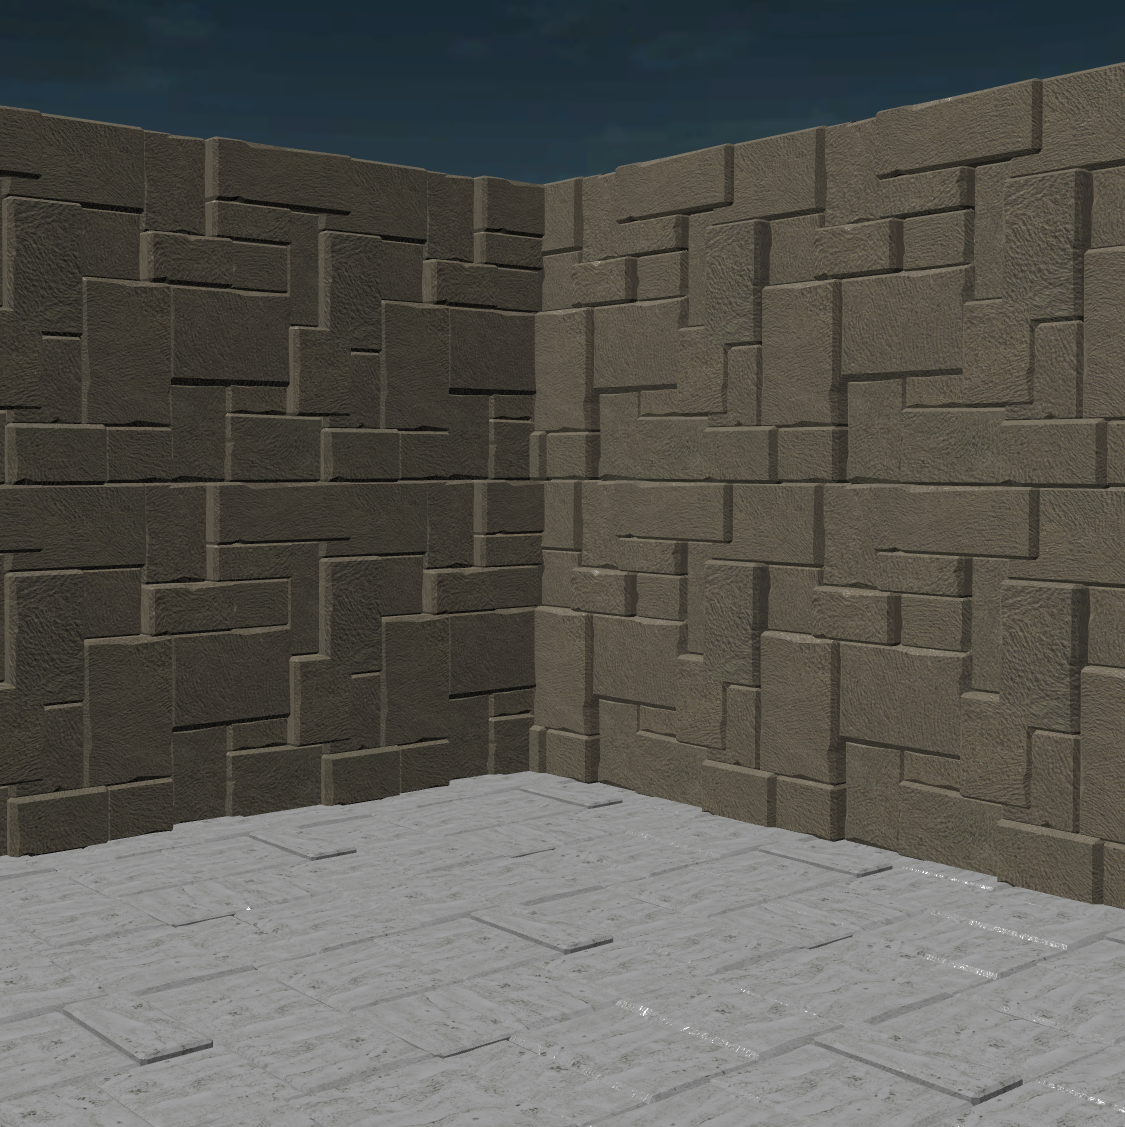
\includegraphics[width=150pt]{images/ch4/floor-walls.png}
    \caption{Floor and walls}
\end{wrapfigure}

The setting of the game is a ceiling-less labyrinth that represents the ruins of some castle-like building. It is built for the most part with two elements, which are the \textit{floor} and the \textit{wall}.
These two elements are modular tiles that can be replicated through instancing to build larger surfaces. We organized the dungeon in a grid of \textit{blocks}, each 6 units long and wide and 4 units high. Since both modular tiles are 2x2 units, this results in each floor block being composed of 3x3 tiles and each wall segment being made of 3x2 tiles. We created an \texttt{addBlock} function to create a floor block and any number of wall segments surrounding it with one line of code, and we used it to build rooms and corridors.

When we had finished designing the final version of the dungeon layout and implemented it in code, we found out during the testing phase that we were loading too many objects at the same time in the same scene, and as a result the framerate, especially on lower-hardware platforms, was not ideal. For this reason, we changed the design of the dungeon and we split it into different parts, each being a separate scene. In this way we could load fewer elements and obtain a more stable gameplay.

As a consequence of the division of the dungeon into 5 different sections, we had to implement a system to move the protagonist from one to another.
The loading of the different scenes happens when the player interacts with a door.

\begin{wrapfigure}[10]{r}{0.5\textwidth}
    \centering
    \vspace{-15pt}
    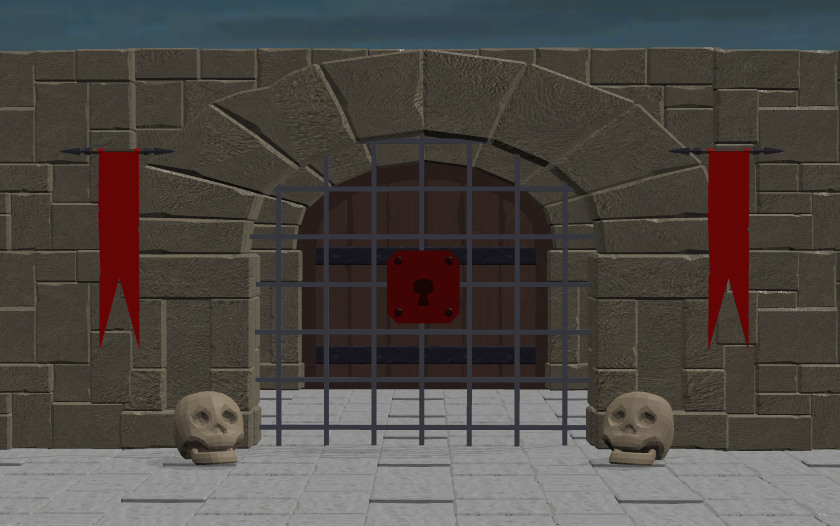
\includegraphics[width=170pt]{images/ch4/red-entrance.png}
    \caption{Red dungeon area entrance}
\end{wrapfigure}

The dungeon areas other than the initial one will be here on referred to by using their color. The first three areas that can be accessed from the spawn have been arbitrarily assigned the colors yellow, green and blue. These colors can be found on the corresponding keys and padlocks used to access that particular area, and on the banners on the walls in front of and inside them. The last area is the boss room, and its color is red.

\newpage

Another solution we adopted for improving the performance in-game was to edit wall and floor files in Blender, and remove all the faces that are not visible from the camera's perspective. By doing this, we effectively halved the numbers of triangles of the two most common objects of the game.

Finally, a number of purely decorative elements are scattered throughout the dungeon: chairs and tables, cobwebs, skulls, chests, banners - of different colors, and many more.

\begin{figure}[H]
      \centering
      \subfloat{
        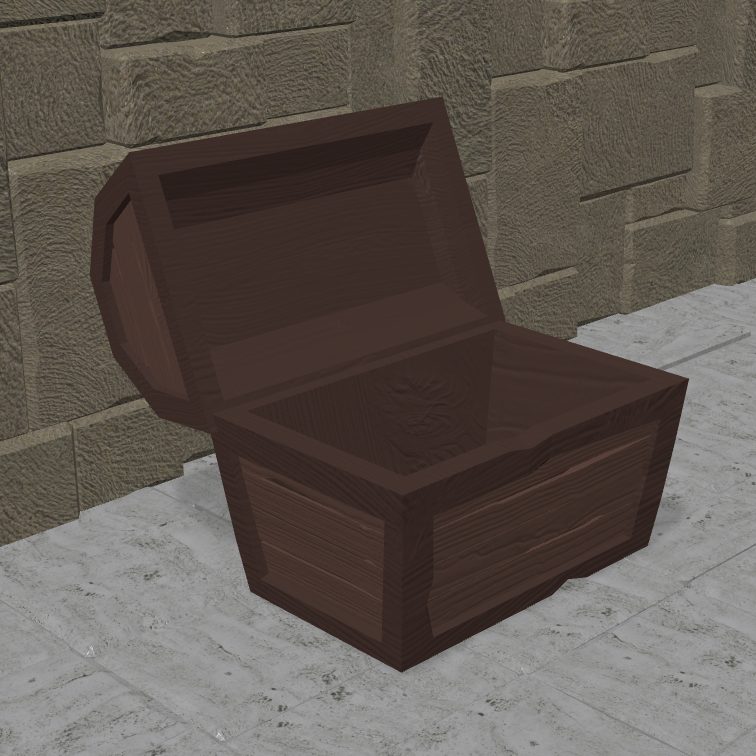
\includegraphics[width=0.35\textwidth]{images/ch4/chest.png}
    }
    \hspace{1cm}
    \subfloat{
        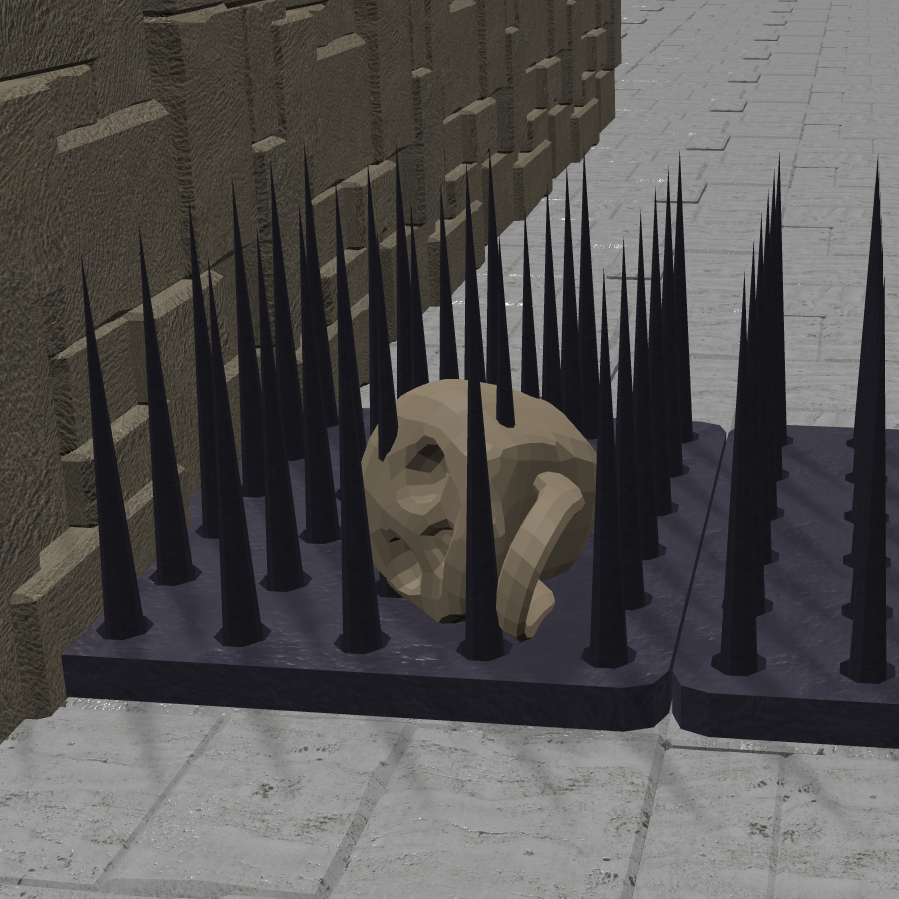
\includegraphics[width=0.35\textwidth]{images/ch4/spikes.png}
    }
\end{figure}

\begin{figure}[H]
      \centering
      \subfloat{
        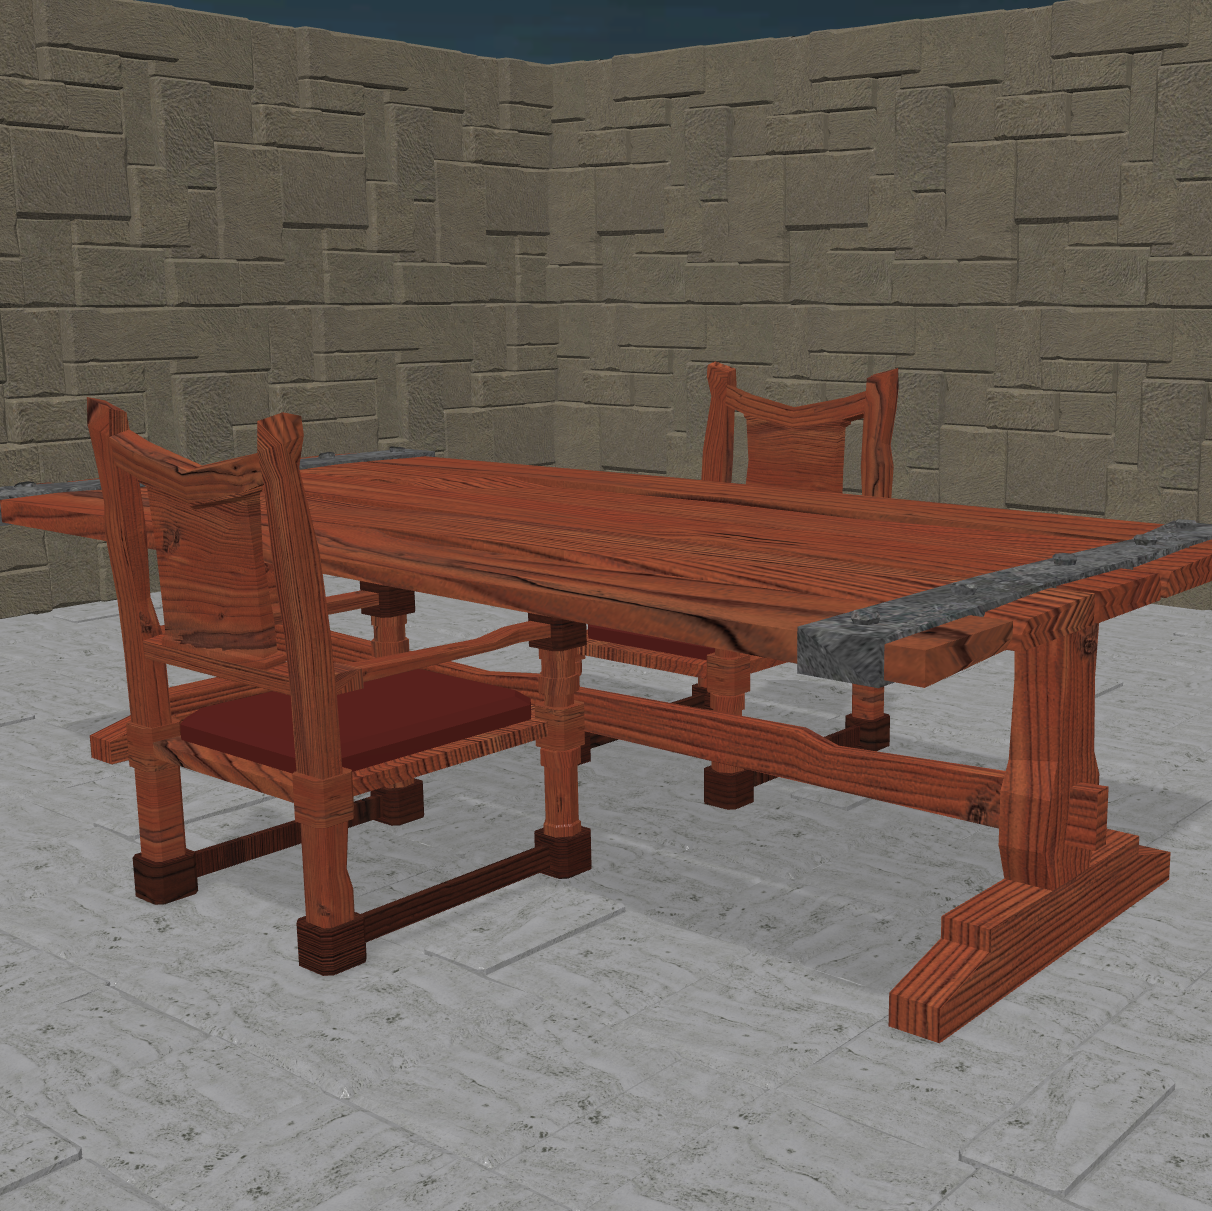
\includegraphics[width=0.35\textwidth]{images/ch4/table-chairs.png}
    }
    \hspace{1cm}
    \subfloat{
        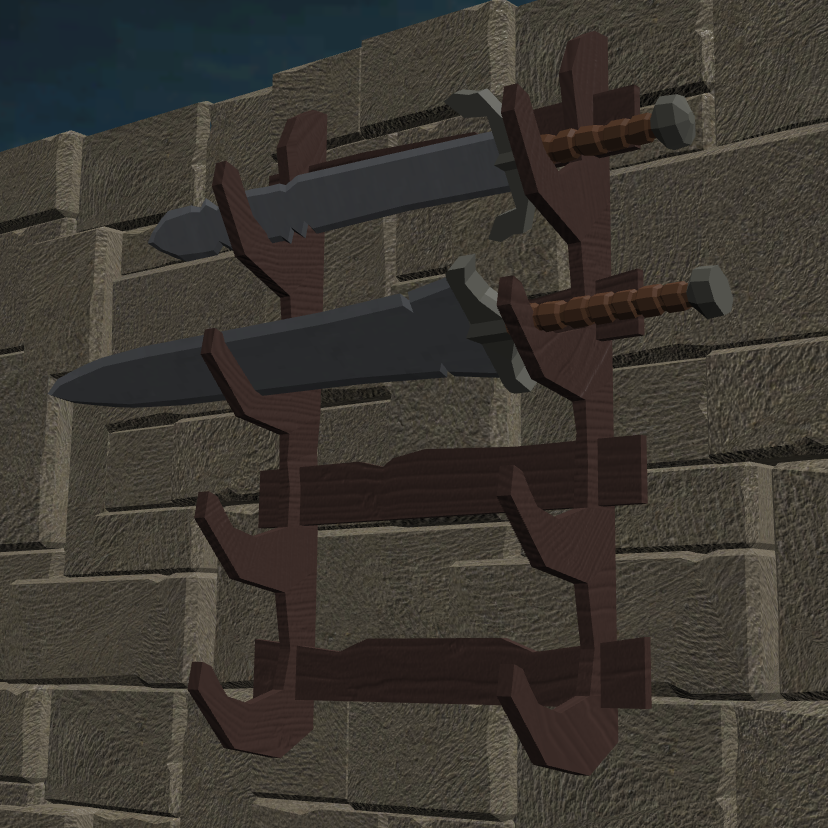
\includegraphics[width=0.35\textwidth]{images/ch4/swords.png}
    }
    \caption{Some of the elements present in the game}
\end{figure}

\section{The battle scene}

The battle scene is the place where the player character is transported to when he interacts with an enemy.
Essentially it's a small square room built in the same way as the dungeon, containing some decorative elements and, of course, the two fighters.

This scene also includes a graphical interface to show the state of the battle and handle user interaction:

\begin{itemize}
    \item On the top left and top right corners, two panels show the remaining HP of the player and enemy respectively, as well as the player's charge state. They are updated each frame.
    \item On the bottom left during the player turn, the four action buttons and the text box explaining the currently selected button are shown. The \textit{Fireball} and \textit{Prayer} buttons are enabled or disabled depending on the player character's charge state: they can only be used when the player is charged up. The text box is managed by holding a separate "hovered" boolean flag for each button which is changed through pointer enter/leave events, and choosing which text to show based on those flags, since using those events to directly change the text in the text box would sometimes have concurrency issues. Furthermore, the text box's return to the default prompt when no button is hovered is slightly delayed, so the user can move the cursor from one button to another without the default text flashing for a split second.
    \item On the bottom right corner there is a button to lock or unlock the battle camera. While unlocked, the user can orbit the camera via drag-and-drop; while locked, the camera simply stops accepting such inputs.
\end{itemize}

\begin{figure}[H]
    \centering
    \subfloat{
        \includegraphics[width=0.9\textwidth]{images/ch4/battle-scene.png}
    }
    \caption{The battle scene}
\end{figure}

\section{Ending}

This scene is already fully discussed in the other chapters of this report and has no noteworthy technical details.

\begin{figure}[H]
    \centering
    \subfloat{
        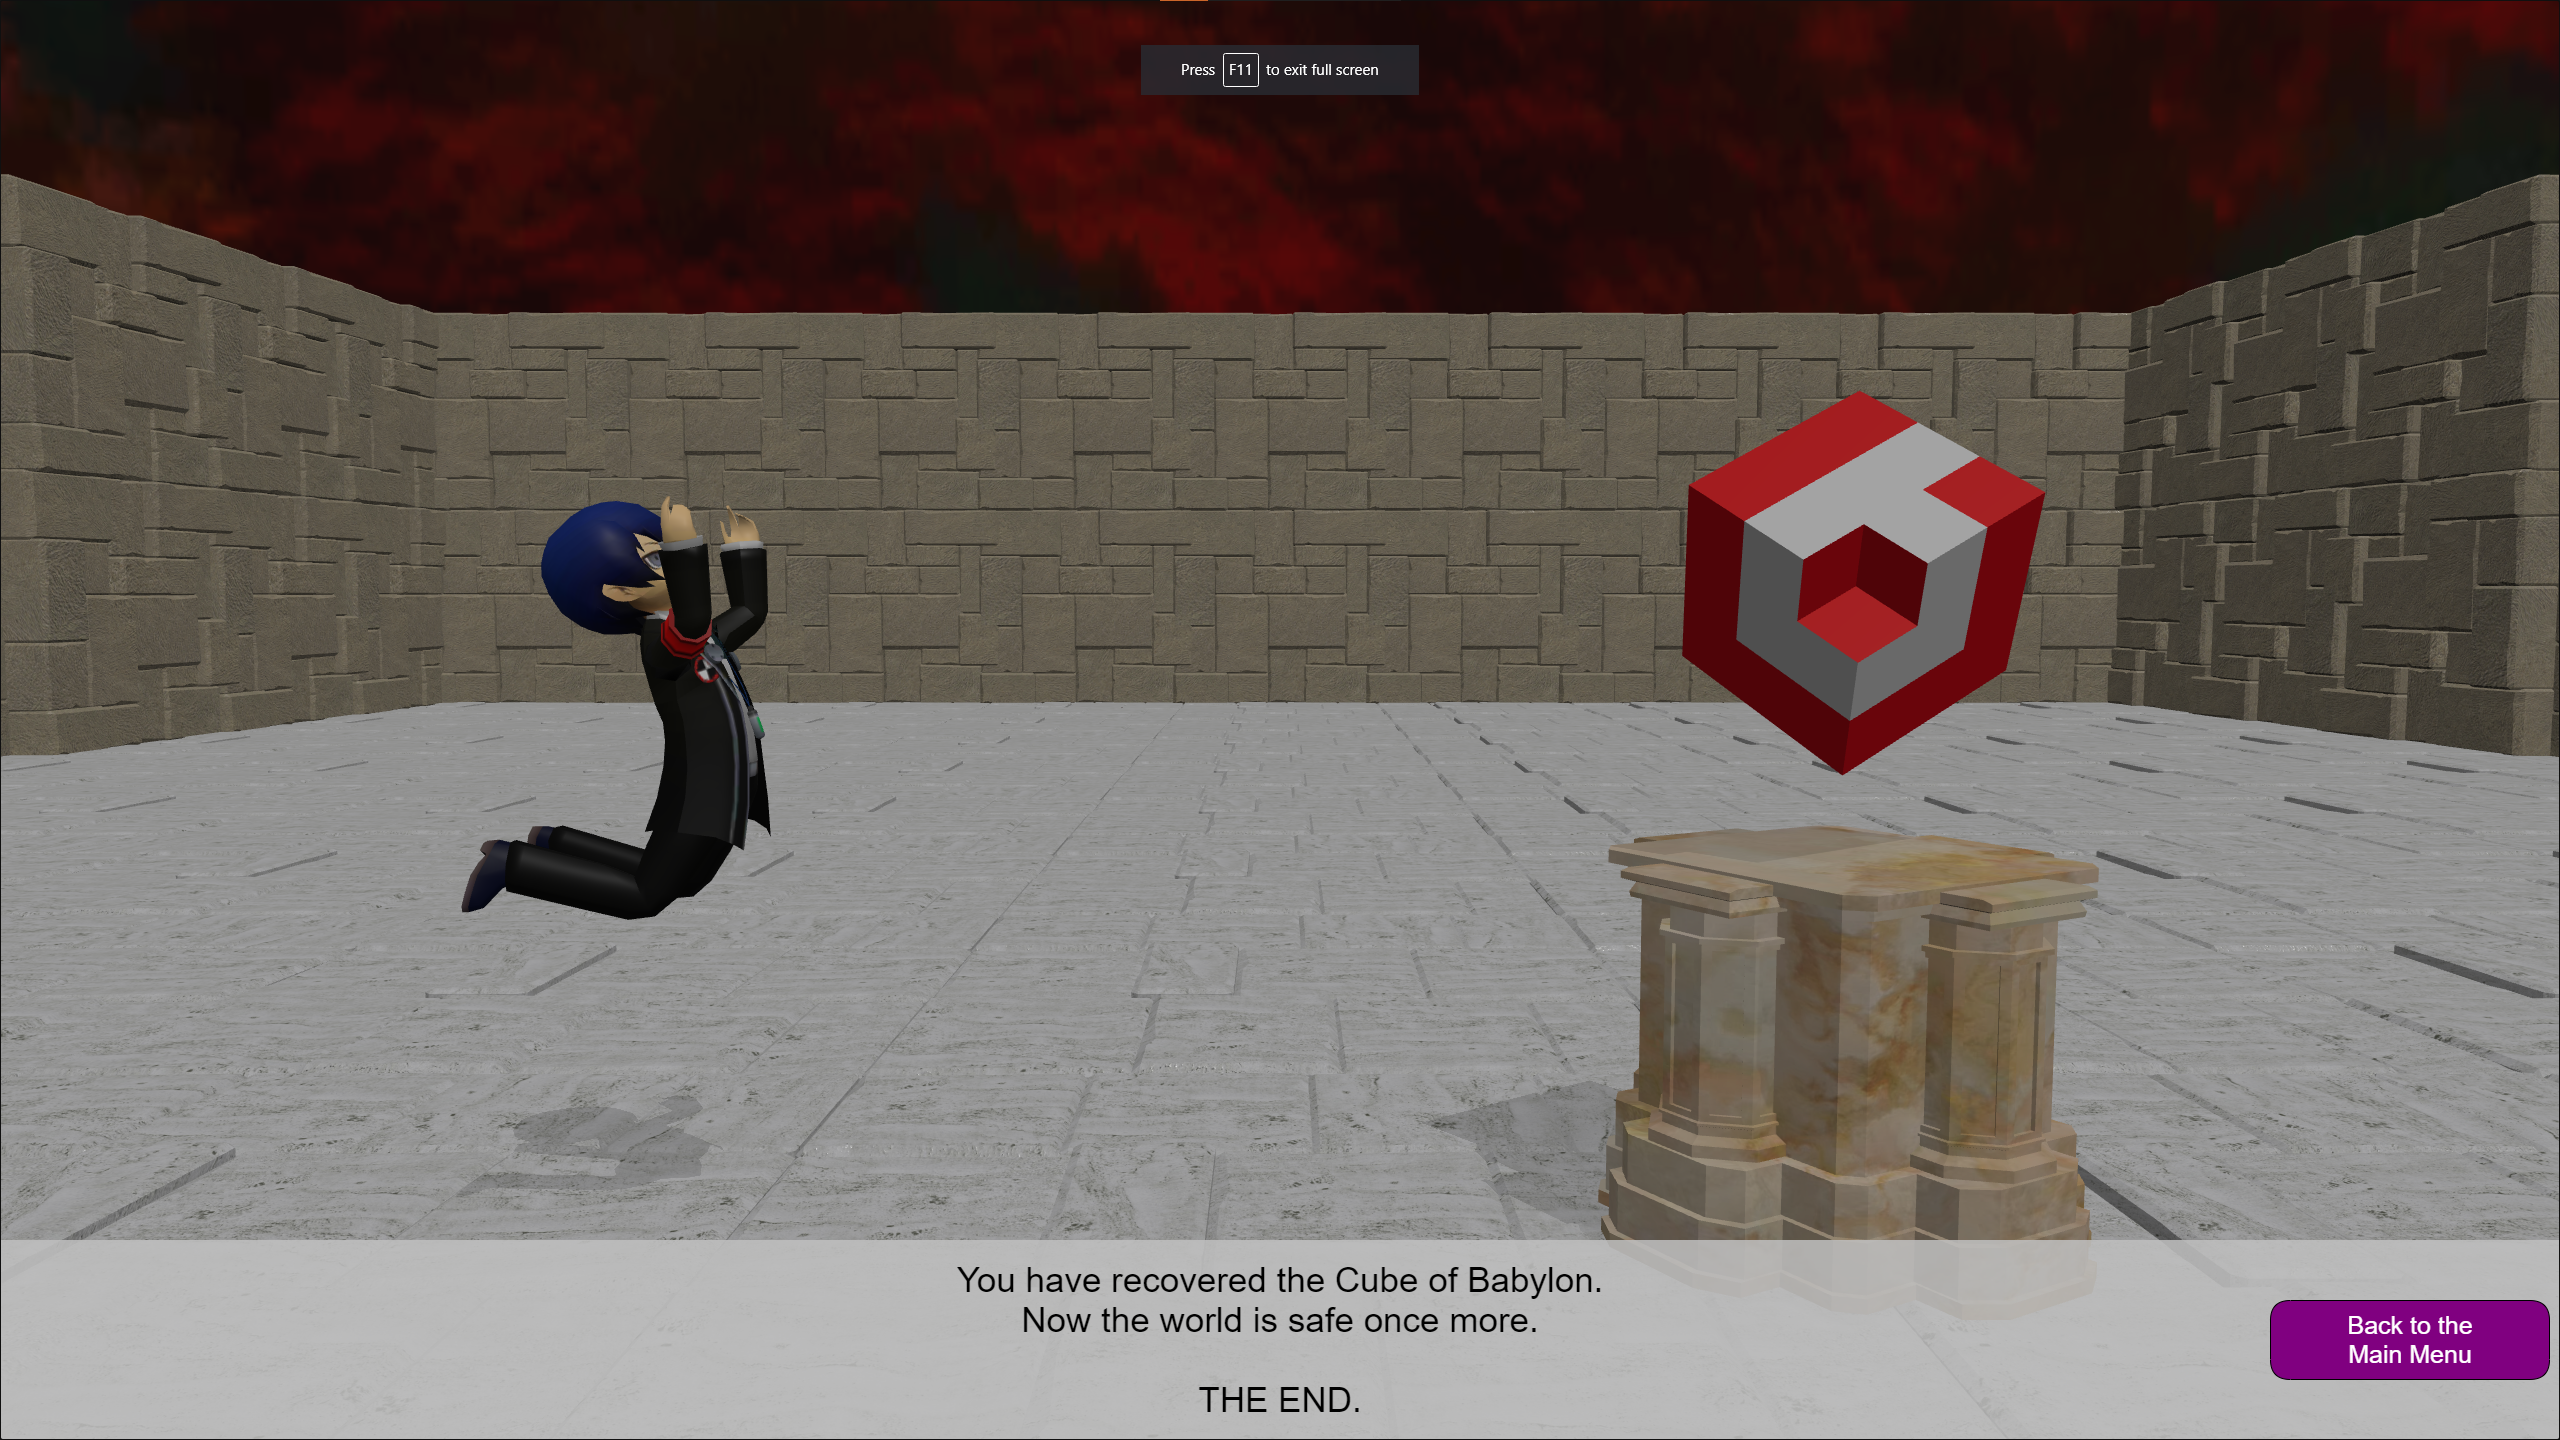
\includegraphics[width=0.9\textwidth]{images/ch4/ending.png}
    }
    \caption{The ending scene}
\end{figure}

\section{Sky maps}
The sky maps are implemented using \texttt{BABYLON.PhotoDome} function, which creates a large sphere around the scene and attaches an equirectangular texture to its internal surface in order to create the illusion of a sky (or fog effect, if one wanted). There are two different images used in the game: the first one is used in most dungeon and battle scenes, while the second one is reserved for the boss.

\begin{figure}[H]
    \centering
    \subfloat{
        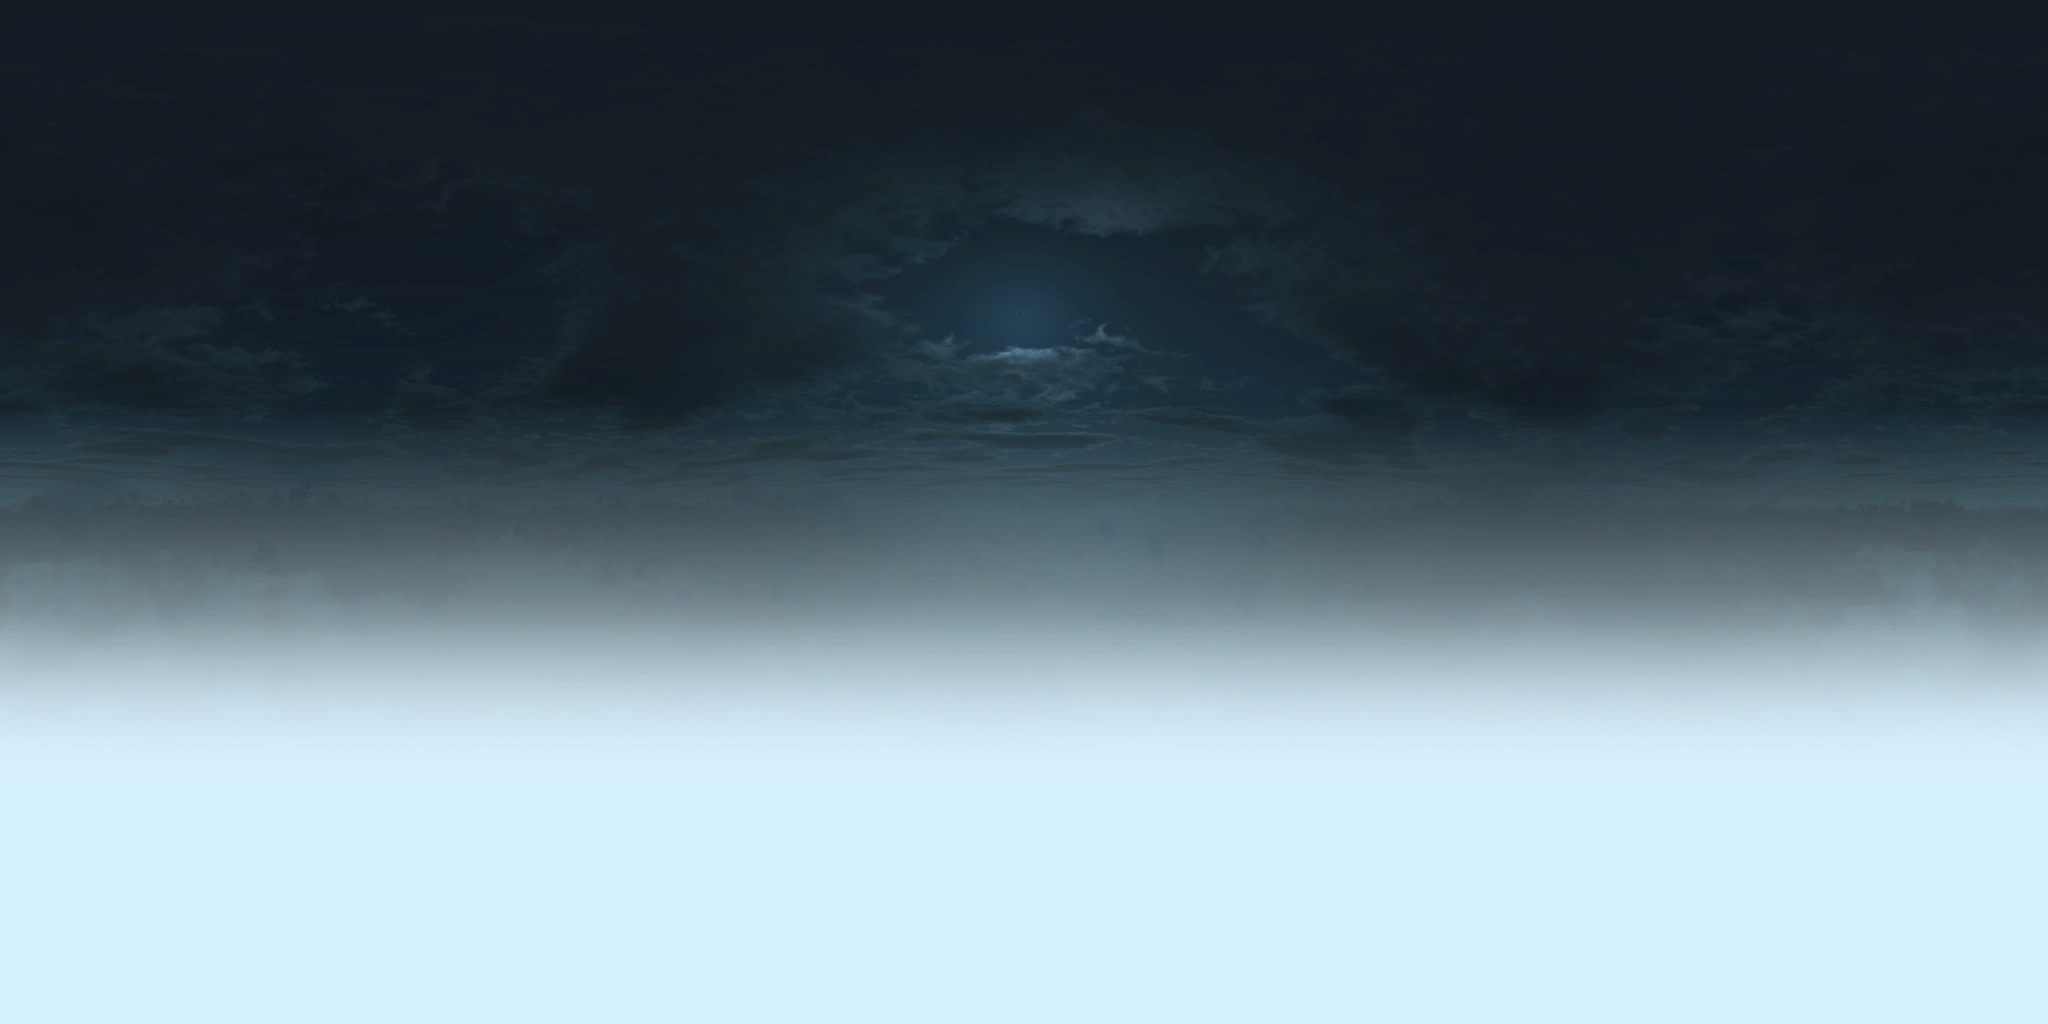
\includegraphics[width=0.9\textwidth]{images/ch4/skybox-dungeon.png}
    }
    \caption{The main sky map used in the dungeon and battle scenes}
\end{figure}

\begin{figure}[H]
    \centering
    \subfloat{
        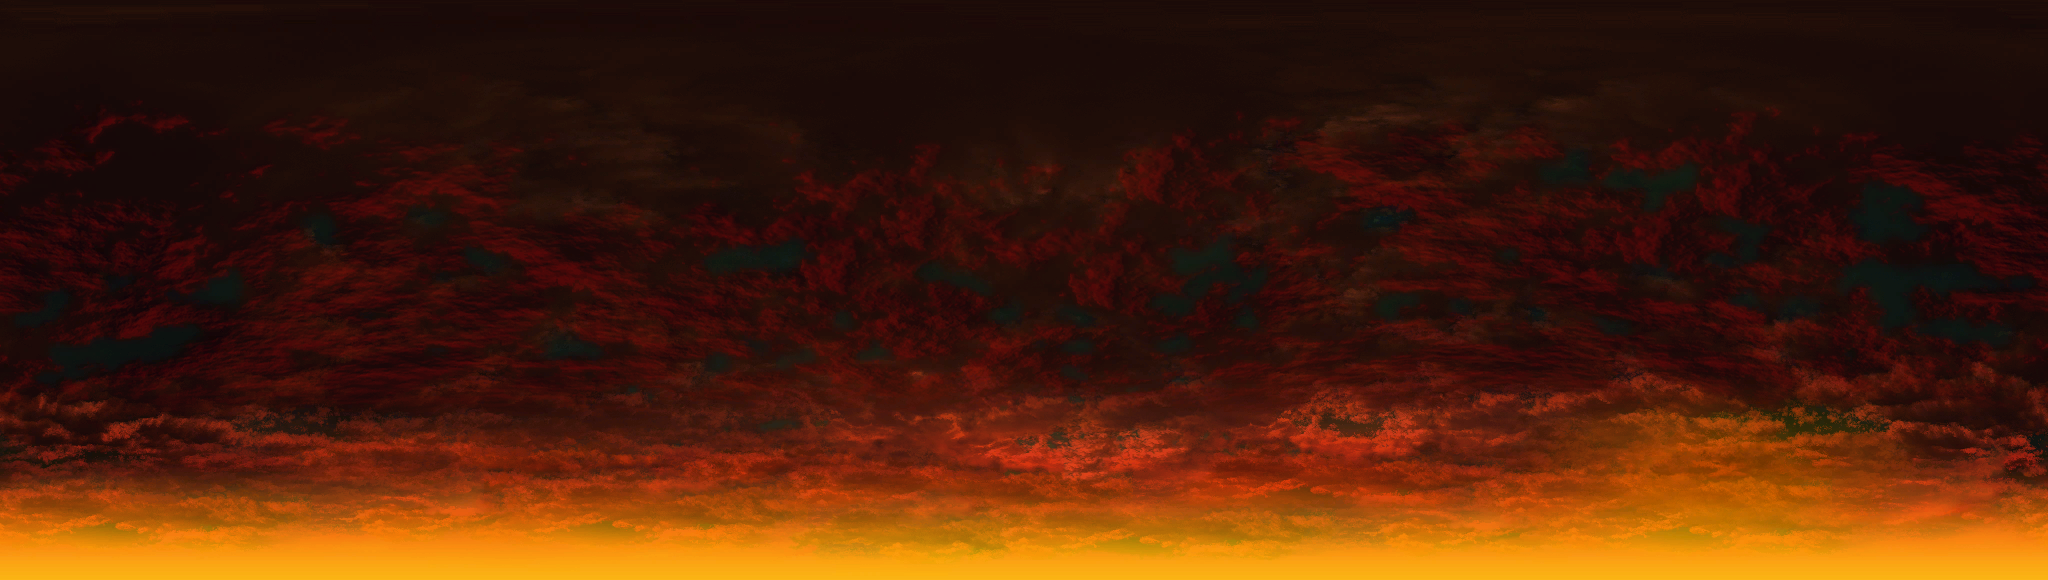
\includegraphics[width=0.9\textwidth]{images/ch4/skybox-boss.png}
    }
    \caption{The boss sky map}
\end{figure}

\section{Camera and movement}

\subsection{Dungeon}

The camera used in the dungeon is a \texttt{Babylon.UniversalCamera}, which is a Babylon element we used to create a first-person perspective.
This camera is moved by the player using keyboard inputs, in two different ways: either using \textit{WASD} or the arrow buttons (see \autoref{sub:exploration-controls}).
The mouse is used to rotate the camera by clicking and dragging.
A gravity force has been applied to the camera, to forbid the player from flying.
The use of the function \texttt{engine.getDeltaTime()} when defining that character walking and running speed assures that all players experience the game moving at the same speed, independently of their framerate.

\subsection{Battle}
The camera used in the dungeon is a \texttt{Babylon.ArcRotateCamera}. The main difference from the dungeon camera is that this can only be rotated around a fixed point located in the center of the scene.
For this reason the keyboard here has no function, and only the mouse is used for rotating.
The camera's latitudinal movement is limited so that it doesn't go underground.
The UI also gives the player the possibility to lock the camera in its initial orientation.

\section{Collisions}
Most elements in the dungeon represent solid objects, so the player should be able to collide with them. However, because most meshes have a complex shape, we found it simpler and more reliable to assign invisible \textit{collision boxes} to those objects. They are simple invisible cuboids created with Babylon's \texttt{Box} primitive with dimensions similar to those of the associated object; they are then \textit{parented} to that object in order to inherit any displacement, rotation and scaling.

By creating flat boxes around the complex objects, and checking collisions with the former rather than the latter, the movement of the player in contact with other objects is smoothed significantly. In particular, the player never trips over all the irregularly-placed bricks of the floor, nor do they get stuck in wall corners.

In order to collide with these boxes, the player camera needs to have a collider as well, to simulate the body of the player. We set up an ellipsoid shape for this purpose.

Our usage of collisions has one basic principle: to stop the player from going where they shouldn't. In the case of walls and floors, they prevent them from falling outside of the map; in other cases, e.g. the locked gates and the spikes in the green room, collision is used as a game mechanic to prevent the player from "sequence breaking" the game. Even the enemies create an invisible collidable box that takes up a whole block for the same reason.
